\documentclass{article}
\usepackage{iclr2027_conference,times}

\usepackage{amsmath,amssymb,amsthm}
\usepackage{booktabs}
\usepackage{multirow}
\usepackage{graphicx}
\usepackage{microtype}
\usepackage[most]{tcolorbox}
\usepackage{xcolor}
\usepackage{tikz}
\usetikzlibrary{arrows.meta,positioning,decorations.pathmorphing}
\usepackage[colorlinks=true,linkcolor=blue,citecolor=blue]{hyperref}
\usepackage{url}

% ---------------------------------------------------------------- macros ----
\newcommand{\E}{\mathbb{E}}
\newcommand{\ind}[1]{\mathbf{1}\!\left[#1\right]}
\newcommand{\sg}{\mathrm{sg}}
\newcommand{\cube}{c}
\newcommand{\Reach}{\mathrm{reach}}
\newcommand{\Visit}{\mathrm{visit}}
\newcommand{\Nhat}{\hat N}

\newtheorem{proposition}{Proposition}

\definecolor{findingframe}{HTML}{2F4858}
\definecolor{findingback}{HTML}{F2F6F8}
\newtcolorbox{finding}[1][]{
  enhanced, breakable,
  colback=findingback, colframe=findingframe,
  boxrule=0.4pt, left=6pt, right=6pt, top=5pt, bottom=5pt,
  fonttitle=\bfseries\footnotesize,
  coltitle=white,
  attach boxed title to top left={yshift=-2mm, xshift=4mm},
  boxed title style={colback=findingframe, boxrule=0pt, sharp corners},
  title={Finding}, #1
}

\title{Making Successor Measures Work for Robot Manipulation}
\author{Anonymous}

% Uncomment for the camera-ready version.
% \iclrfinalcopy

\begin{document}
\maketitle

% ============================================================================
\section{Introduction}
\label{sec:introduction}

This paper studies a concrete failure of zero-shot reinforcement learning.
Forward--backward (FB) representations \citep{touati2021learning,touati2023does}
learn a successor measure --- the discounted state occupancy of a family of
policies --- so that any reward specified at test time can be turned into a
value function and a policy without further training. FB was developed and
validated on exploratory locomotion and navigation data (ExoRL-style
unsupervised exploration; maze navigation), where it works well. On offline
robot \emph{manipulation} it breaks at the first step: on OGBench cube
manipulation \citep{park2024ogbench}, tuned FB reaches $0.42$ success while
goal-conditioned IQL \citep{kostrikov2021offline} with the same dataset, the
same actor class, and the same bilinear critic reaches $0.93$. We trace this
gap to a structural property of manipulation \emph{play data} that the domains
FB was tested on do not have, and we repair the pipeline piece by piece. Our
contributions:

\begin{enumerate}
    \item \textbf{A data-level diagnosis} (\S\ref{sec:playdata}). Manipulation
    play data is \emph{revisit-dominated}: the manipulated object is exactly
    stationary on $48\%$ of all transitions (median $44$ consecutive steps),
    so discounted occupancy concentrates near-atomically at the object's
    resting positions --- on our data, occupancy after first arrival averages
    $\approx\!25$ discounted visits and carries essentially no control signal.
    FB's objective regresses the occupancy \emph{density}, whose Bellman
    target does not exist at exactly these concentrated pairs; we show the
    resulting instability on a \emph{frozen} representation that already
    supports $0.97$ control ($350\times$ scale growth without the
    orthonormality term; success capped at $0.23$ with it).
    \item \textbf{A curriculum that fits the data} (\S\ref{sec:bounded}).
    Querying a small goal region turns the objective into goal-conditioned TD
    with a sparse indicator reward. The revisit structure then motivates a
    two-phase curriculum: first train the \emph{absorbing} (first-visit)
    backup --- the factor that carries the control signal --- then add the
    revisit mass by switching to the non-absorbing backup, warm-started, with
    the goal representation frozen.
    \item \textbf{An object that is a measure} (\S\ref{sec:measure-validity}).
    Task success does not certify a measure, so we evaluate the occupancy
    object directly. The raw object carries $24$--$29\%$ negative mass; a
    non-negativity penalty alone inflates total mass $2.5$--$3.6\times$;
    pairing it with a mass-conservation penalty derived from an exact
    occupancy identity fixes sign and scale together ($<1.5\%$ negative mass,
    calibration and control unchanged).
    \item \textbf{Zero-shot evaluation on both axes}
    (\S\ref{sec:results}, \S\ref{sec:reward-transfer}). A single comparison
    (Table~\ref{tab:main}) spans goal-reaching tasks and $48$ constructed
    held-out rewards. The final method beats the matched anchor on every
    goal-reaching environment and earns $2.5\times$ FB's return on held-out
    rewards; two further repairs --- an importance weight for return
    prediction and reward-derived task vectors for policy coverage --- account
    for the remaining transfer failures.
\end{enumerate}

The one input we do not learn is the region itself: a three-dimensional object
position and a $4$\,cm radius, supplied from the benchmark. An ablation shows a
correlated but non-evaluated region (end-effector position) retains most of the
benefit, so the requirement is region structure rather than the privileged
variable; discovering that structure from data is open.

% ============================================================================
\section{Preliminaries}
\label{sec:prelim}

\paragraph{Goal-conditioned RL.}
We consider a Markov decision process with state space $\mathcal{S}$, action
space $\mathcal{A}$, transition kernel $P$, and discount $\gamma\in(0,1)$. In
goal-conditioned RL, a goal $g$ defines the sparse reward
$r_g(s')=\ind{s'\in S_g}$ for some goal set $S_g$, and the standard
goal-reaching value of a policy $\pi$ is $\E_\pi[\gamma^{T_g}]$, where $T_g$ is
the hitting time of $S_g$
\citep{kaelbling1993learning,andrychowicz2017hindsight}. Offline, the agent
learns from a fixed dataset of transitions; hindsight relabeling supplies goals
from observed states.

\paragraph{Successor measures.}
The successor measure of $\pi$ is its discounted state occupancy, viewed as a
measure over sets $X\subseteq\mathcal{S}$:
\begin{equation}
\label{eq:sm}
M^{\pi}(s,a,X)
=
\E_{\pi}\!\Big[
\sum_{t\ge 0}\gamma^{t}\ind{s_{t+1}\in X}
\,\Big|\,
s_{0}=s,\,a_{0}=a
\Big].
\end{equation}
Intuitively, $M^\pi(s,a,X)$ counts the discounted time the policy will spend in
$X$. Its usefulness is that any reward's value is an integral against it,
$Q_r^{\pi}(s,a)=\int r(x)\,dM^{\pi}(s,a,x)$: dynamics are learned once, rewards
are supplied later \citep{dayan1993improving,blier2021learning}.

\paragraph{Forward--backward representations and zero-shot RL.}
FB methods \citep{touati2021learning,touati2023does} factorize the successor
measure's density with respect to a reference distribution $\rho$ (in practice,
the dataset marginal):
\begin{equation}
\label{eq:fb}
M^{\pi_z}(s,a,X)
\approx
\int_X F(s,a,z)^{\top}\psi(x)\,d\rho(x).
\end{equation}
Here $z$ is a task vector indexing a family of policies $\pi_z$, and $x$ is a
query state, independent of $z$. At test time, a reward $r$ observed on dataset
samples is converted to a task vector by least-squares reward inference,
$z_r \propto \E_{x\sim\rho}[r(x)\psi(x)]$, and the agent acts greedily on
$Q_r(s,a)\approx F(s,a,z_r)^{\top}z_r$ with no further training. This is the
zero-shot RL protocol we evaluate throughout.

\paragraph{Setting.}
We use OGBench state-based manipulation \citep{park2024ogbench}, primarily
\texttt{cube-single-play-v0}: a $6$-DoF arm, one cube, $28$-dimensional states,
and $10^6$ offline transitions of scripted play that repeatedly picks the cube
up, carries it, and sets it down. No benchmark reward labels are used to fit
any of our objectives. The method is given a state abstraction
$\cube(x)\in\mathbb{R}^3$ (cube position) and a radius $\epsilon=4$\,cm, which
define goal regions
$B_\epsilon(g)=\{x:\|\cube(x)-\cube(g)\|\le\epsilon\}$. This is a substantive
assumption --- three of twenty-eight state dimensions, at the benchmark's own
tolerance --- and we quantify what it contributes in \S\ref{sec:results}.

\paragraph{Protocol.}
Unless stated otherwise: rank-$50$ bilinear critic $F^\top\psi$, twin heads
with a minimum target, $\gamma=0.99$, hindsight-relabeled batch goals (a batch
of $n$ transitions yields an $n\times n$ matrix of state--goal pairs), a
flow-matching behavior-cloning actor with one-step distillation, $500$k
gradient steps, $2$--$3$ seeds per cell. \emph{Task success} means the
benchmark's goal-conditioned evaluation, averaged over its five tasks with $50$
episodes each. Measure-side evaluations (Monte-Carlo occupancy comparisons,
reward-transfer harnesses) are defined where they are used.

% ============================================================================
\section{The problem: play data is revisit-dominated, and densities cannot
absorb that}
\label{sec:playdata}

What is different about manipulation play data? In the domains where FB was
developed --- unsupervised-exploration locomotion and maze navigation --- the
outcome variable is the agent's own configuration, and it changes at
essentially every step: a walker's joints never stop, a maze agent keeps
moving. Occupancy under such data is \emph{diffuse}. Manipulation play data is
the opposite. The outcome variable is the \emph{object's} position, and the
object only moves while grasped.

\begin{figure}[t]
\centering
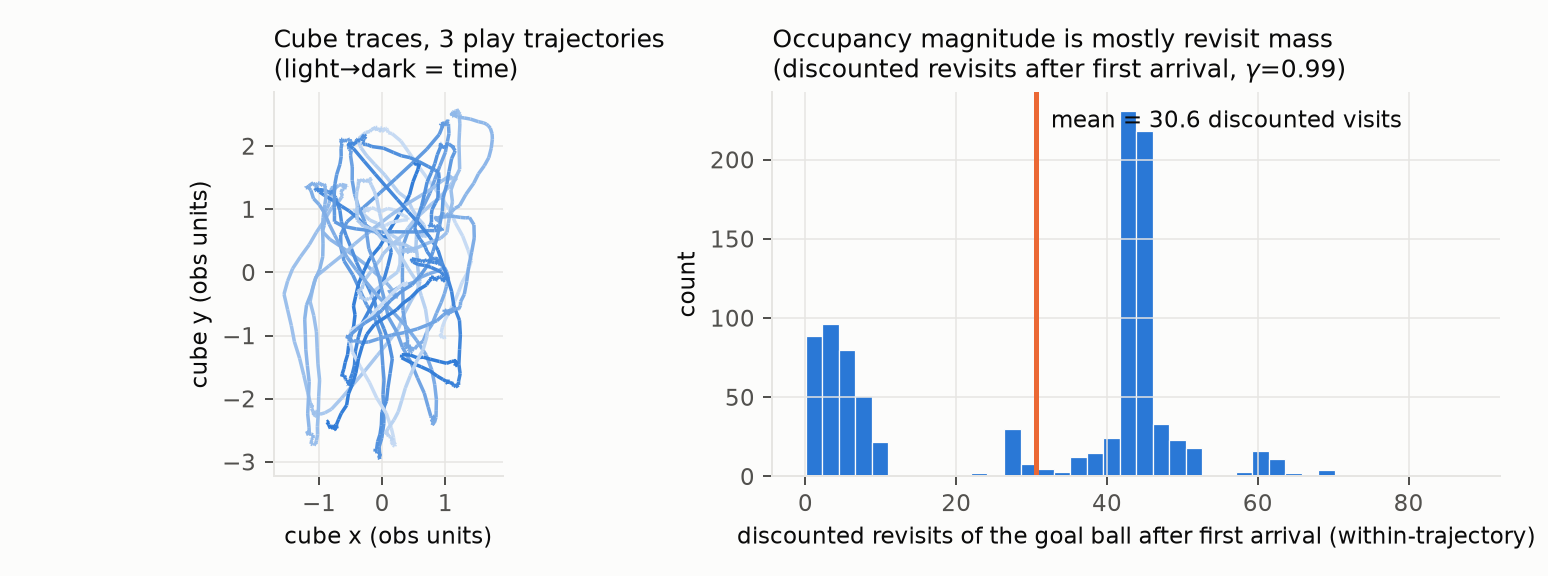
\includegraphics[width=0.95\textwidth]{figures/playdata.png}
\caption{Manipulation play data is revisit-dominated. \emph{Left:} cube traces
of three play trajectories --- the cube rests, is carried, and rests again.
\emph{Right:} discounted occupancy of a $4$\,cm goal ball accumulated
\emph{after} its first arrival (within-trajectory Monte Carlo, $\gamma=0.99$):
the mean is $30.6$ discounted visits, out of a maximum possible
$1/(1-\gamma)=100$. Most of the magnitude of the successor measure on this
data is revisit mass, not first-arrival mass.}
\label{fig:playdata}
\end{figure}

Concretely, on \texttt{cube-single-play-v0} (Figure~\ref{fig:playdata}): the
cube position is bit-identical across $48\%$ of all transitions, with a median
stationary run of $44$ consecutive steps; a $4$\,cm ball around a random
dataset state contains only $1.3\%$ of the data, yet the discounted occupancy
a trajectory accumulates in that ball \emph{after first arriving} averages
$25$--$31$ visits out of a possible $100$. Moreover this revisit mass is close
to a function of the goal alone: a goal-only regressor predicts Monte-Carlo
occupancy at rank correlation $0.60$--$0.63$, while the first-arrival term
alone predicts at $0.06$. In other words, on play data the successor measure's
\emph{magnitude} is dominated by dwelling and revisiting --- a component that
carries almost no information about which action to take now --- while the
control signal lives in the small first-arrival factor.

The structure strengthens with every additional object, because play
manipulates one object at a time while every other object rests. On
\texttt{cube-double-play-v0}, each cube is stationary on $72\%$ of transitions
and revisit mass averages $32$; on \texttt{scene-play-v0}, the drawer and
window are stationary on $91\%$ of transitions, the buttons on $99.6\%$, and
revisit mass averages $37$ --- while the conjunctive goal region (all objects
in place) covers only $0.03$--$0.4\%$ of the data
(Appendix~\ref{app:playstats}). If the revisit mechanism is right, methods
built on occupancy densities should degrade \emph{most} where revisit
dominance is highest --- and they do: FB scores $0.42$ on \texttt{cube-single}
but $0.05$ on \texttt{scene} (Table~\ref{tab:main}).

This structure is precisely what a pointwise density objective cannot absorb.
Write $m_z(s,a,x)=dM^{\pi_z}(s,a,\cdot)/d\rho(x)$ for the successor density
that FB factorizes as $F^{\top}\psi$. Its Bellman equation is
\begin{equation}
\label{eq:density-bellman}
m_z(s,a,x)
=
\E_{s'}\Big[
\tfrac{\delta_{s'}(x)}{\rho(x)}
+\gamma\,\E_{a'\sim\pi_z}\,m_z(s',a',x)
\Big].
\end{equation}
The immediate term is the density of a point mass at the observed successor:
zero for $x\ne s'$ and unbounded at $x=s'$. There is no finite number a critic
can output at the observed successor that makes the squared TD error small.
Revisit-dominated data makes this worst case typical: when the object rests,
the same successor recurs for dozens of steps, and the true occupancy
approaches an atom --- the density the objective is asked to represent grows
without bound exactly where the data concentrates. A tabular construction with
play-data anatomy reproduces the estimator gap with no neural networks
(Appendix~\ref{app:playpen}).

Standard FB works around the singular term with a surrogate loss
\citep{touati2021learning},
\begin{equation}
\label{eq:fb-loss}
\mathcal{L}_{\mathrm{FB}}
=
\tfrac{1}{2}\E_{x\sim\rho}\big[(m_z-\gamma\bar m_z)^2\big]
-\E\big[m_z(s,a,s')-\gamma\bar m_z(s,a,s')\big]
+\lambda_{\mathrm{ortho}}\mathcal{L}_{\mathrm{ortho}}.
\end{equation}
This has the structure of a contrastive objective: random query states are
negatives and receive a squared residual, while the observed successor is the
positive pair and receives a term that rewards increasing its score
\citep{eysenbach2022contrastive}. But where a contrastive loss saturates its
positive term (through a log-sigmoid), the term here is \emph{linear}:
increasing the matched score always reduces the loss, at any scale --- and on
revisit-dominated data the matched pairs recur relentlessly. The only component
of the objective that opposes the growth is the orthonormality penalty on
$\psi$, a constraint on representation geometry acting as an implicit
normalizer.

\paragraph{Both predicted failures occur, on a frozen representation.}
To rule out representation quality as an explanation, we freeze $\psi$ at a
checkpoint that already supports $0.97$ task success and train only the density
estimator on top of it. Without the orthonormality term, the critic's scale
grows from $154$ to $5.4\times10^4$ within $65$k steps and success decays
$0.98\to0.60\to0.42$ by $100$k across three seeds (Figure~\ref{fig:diverge});
letting $\psi$ train merely accelerates the collapse ($0.97\to0.07$ by $50$k).
With the orthonormality term, scale is stable but success reaches only
$0.225$; a fully tuned FB implementation reaches $\approx0.42$, against
$0.928$ for the matched IQL anchor. The estimator, not the representation, is
the bottleneck.

\begin{figure}[t]
\centering
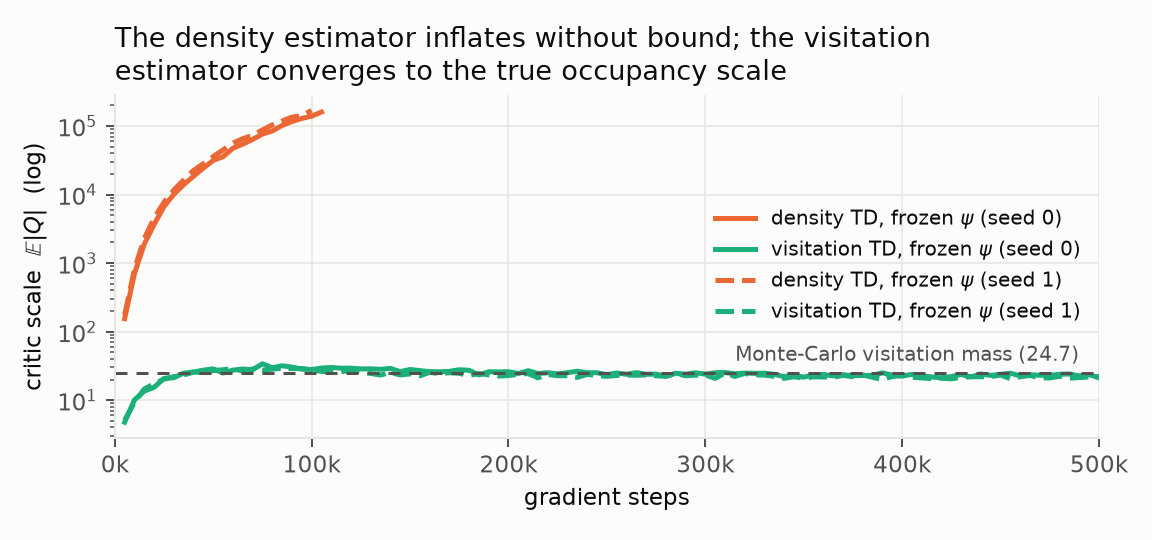
\includegraphics[width=0.62\textwidth]{figures/scale_divergence.png}
\caption{Critic scale $\E|Q|$ (log axis) while training on a \emph{frozen}
backward representation $\psi$. The density surrogate (orange) grows without
bound once the orthonormality term is removed: its linear term always pays for
a larger matched score, and play data supplies the same matched pairs over and
over. The indicator-reward objective of \S\ref{sec:bounded} (aqua) converges to
the Monte-Carlo estimate of the true discounted occupancy (dashed), because
every entry of its TD target is a finite number.}
\label{fig:diverge}
\end{figure}

\begin{finding}
Manipulation play data concentrates occupancy at the object's resting
positions: $48\%$ of transitions leave the cube bit-identical, and revisit mass
after first arrival averages $\approx\!25$--$31$ of a possible $100$ discounted
visits while carrying almost no action information. A pointwise density has no
finite regression target exactly there, and the failure is the objective's, not
the representation's: it occurs with $\psi$ frozen at a checkpoint supporting
$0.97$ control.
\end{finding}

% ============================================================================
\section{The fix: goal-conditioned TD on regions, staged to match the data}
\label{sec:bounded}

The diagnosis dictates the two ingredients of the repair: give every
state--query pair a finite target, and separate the control-bearing
first-arrival factor from the magnitude-bearing revisit mass.

\paragraph{Regions give finite targets.}
Define the indicator reward
\begin{equation}
\label{eq:hit}
h(s',g)=\ind{\|\cube(s')-\cube(g)\|\le\epsilon}\in\{0,1\},
\end{equation}
and regress the region occupancy $M(s,a,B_\epsilon(g))$ instead of the density
$m(s,a,g)$. The immediate term of Equation~\ref{eq:density-bellman} becomes
$h(s',g)$ --- a bounded, sparse, goal-conditioned reward of the kind offline
GCRL trains on routinely. The loss is full-matrix TD regression over the batch,
\begin{equation}
\label{eq:matrix-loss}
\mathcal{L}=\tfrac{1}{n^2}\sum\nolimits_{ij}\big(Q_{ij}-y_{ij}\big)^2,
\qquad
Q_{ij}=F(s_i,a_i,z_j)^{\top}\psi(g_j),
\end{equation}
with no linear term and no orthonormality penalty: the $0/1$ reward supplies
the scale that the penalty previously had to impose. Intuitively, we have
replaced density estimation with policy evaluation.

\paragraph{Two backups, one per factor.}
A finite event admits two TD targets, distinguished by what happens after the
first hit:
\begin{equation}
\label{eq:backups}
y^{\Reach}_{ij}=h_{ij}+\gamma(1-h_{ij})\,\bar Q_{ij},
\qquad\qquad
y^{\Visit}_{ij}=h_{ij}+\gamma\,\bar M_{ij}.
\end{equation}
The first treats the region as absorbing, exactly as in standard
goal-conditioned RL; the second does not, so occupancy keeps accumulating.

\begin{proposition}
\label{prop:fixed-points}
For a fixed continuation policy, both operators in Equation~\ref{eq:backups}
are $\gamma$-contractions in the sup norm, with unique fixed points
\begin{equation*}
Q^{\Reach}(s,a,g)=\E\!\left[\gamma^{T_g}\ind{T_g<\infty}\right],
\qquad
M^{\Visit}(s,a,g)=\E\Big[\sum\nolimits_{t\ge0}\gamma^t h(s_{t+1},g)\Big],
\end{equation*}
where $T_g$ is the hitting time of $B_\epsilon(g)$.
\end{proposition}

Intuitively, these are the two factors that \S\ref{sec:playdata} separated:
$Q^{\Reach}\in[0,1]$ is the standard goal-reaching value --- the small factor
that carries the control signal --- and $M^{\Visit}\in[0,1/(1-\gamma)]$ is the
successor measure of the region, whose magnitude on play data is dominated by
revisit mass. We call them the \textbf{reaching value} and the
\textbf{visitation measure}.

\paragraph{The curriculum.}
The data structure motivates training them in that order. Phase 1 trains the
reaching value with the policy's goal equal to the queried goal: a well-posed
sparse-reward GCRL problem in which every unit of value is control-relevant.
Phase 2 warm-starts from that checkpoint, freezes $\psi$, switches to the
non-absorbing backup, and samples the task $z$ and the query $g$
independently, $M(s,a,z,g)=F(s,a,z)^{\top}\psi(g)$ --- the separated form that
reward integration requires (Equation~\ref{eq:fb}). Phase 2's role is to add
the revisit mass that reward integration needs on top of a goal geometry that
control has already validated. The staging is a design choice grounded in the
data statistics, not a mathematical identity: the factorization
``occupancy $=$ reaching $\times$ recurrence'' that suggests it is exact only
for singleton goals, and its action-independence fails pointwise on regions
(intraclass correlation $0.24$--$0.29$), so phase 2 trains by TD rather than by
multiplying estimated factors.

\begin{figure}[t]
\centering
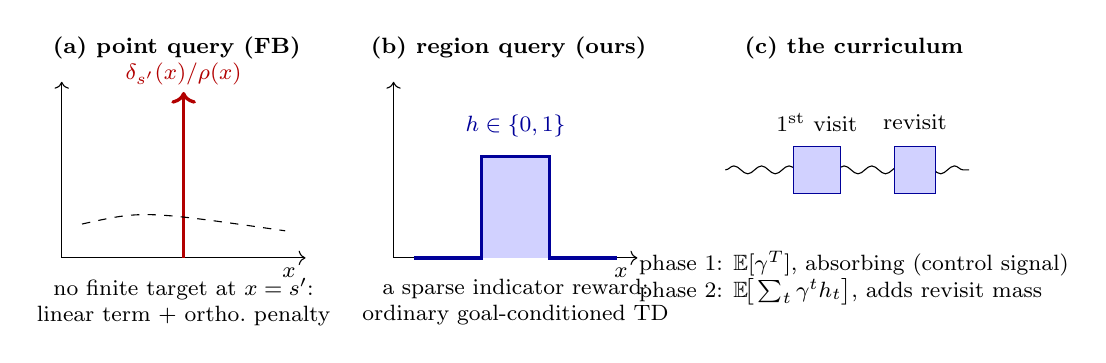
\begin{tikzpicture}[scale=0.86, every node/.style={font=\footnotesize}]
% ---------------- panel (a): point query ----------------
\begin{scope}[xshift=0cm]
\node[font=\footnotesize\bfseries] at (1.7,3.1) {(a) point query (FB)};
\draw[->] (0,0) -- (3.6,0) node[below left] {$x$};
\draw[->] (0,0) -- (0,2.6);
\draw[very thick,red!70!black,->] (1.8,0) -- (1.8,2.45);
\node[red!70!black] at (1.8,2.72) {$\delta_{s'}(x)/\rho(x)$};
\draw[dashed] (0.3,0.5) .. controls (1.2,0.7) .. (3.3,0.4);
\node[align=center] at (1.8,-0.65) {no finite target at $x=s'$:\\
linear term $+$ ortho.\ penalty};
\end{scope}
% ---------------- panel (b): region query ----------------
\begin{scope}[xshift=4.9cm]
\node[font=\footnotesize\bfseries] at (1.7,3.1) {(b) region query (ours)};
\draw[->] (0,0) -- (3.6,0) node[below left] {$x$};
\draw[->] (0,0) -- (0,2.6);
\fill[blue!18] (1.3,0) rectangle (2.3,1.5);
\draw[very thick,blue!60!black] (0.3,0) -- (1.3,0) -- (1.3,1.5) -- (2.3,1.5) -- (2.3,0) -- (3.3,0);
\node[blue!60!black] at (1.8,1.95) {$h\in\{0,1\}$};
\node[align=center] at (1.8,-0.65) {a sparse indicator reward:\\
ordinary goal-conditioned TD};
\end{scope}
% ---------------- panel (c): two backups ----------------
\begin{scope}[xshift=9.8cm]
\node[font=\footnotesize\bfseries] at (1.9,3.1) {(c) the curriculum};
\draw[decorate,decoration={snake,amplitude=.5mm,segment length=3.5mm}]
  (0,1.3) -- (3.6,1.3);
\fill[blue!18] (1.0,0.95) rectangle (1.7,1.65);
\fill[blue!18] (2.5,0.95) rectangle (3.1,1.65);
\draw[blue!60!black] (1.0,0.95) rectangle (1.7,1.65);
\draw[blue!60!black] (2.5,0.95) rectangle (3.1,1.65);
\node at (1.35,2.0) {$1^{\text{st}}$ visit};
\node at (2.8,2.0) {revisit};
\node[align=left] at (1.9,-0.3)
  {phase 1: $\E[\gamma^{T}]$, absorbing (control signal)\\
   phase 2: $\E\!\big[\sum_t\gamma^t h_t\big]$, adds revisit mass};
\end{scope}
\end{tikzpicture}
\caption{(a)~FB regresses a successor density whose empirical target at the
observed successor is a Dirac measure --- no finite prediction is correct
there, so the loss substitutes an unbounded linear term restrained only by an
orthonormality penalty; revisit-dominated play data supplies those matched
pairs constantly. (b)~Querying a region turns the immediate term into a sparse
indicator reward and the objective into standard goal-conditioned TD. (c)~The
curriculum mirrors the data's two factors: train the absorbing first-visit
value first (all control signal), then add the revisit mass by switching to the
non-absorbing backup with the goal representation frozen.}
\label{fig:idea}
\end{figure}

% ============================================================================
\section{Results: goal-reaching tasks and constructed rewards, one table}
\label{sec:results}

Table~\ref{tab:main} is the paper's main comparison. The left column group is
the benchmark's goal-reaching evaluation on three environments. The right group
evaluates zero-shot reward transfer on \texttt{cube-single}: $48$ held-out
rewards over the cube abstraction (\S\ref{sec:reward-transfer};
concentrated $=$ balls at radii $0.4/0.8$ and Gaussians at bandwidth $0.4$;
broad $=$ ball $1.6$ and Gaussian $0.8$; compositional $=$ two disjoint zones).
All rewards take values in $[0,1]$, so with horizon $200$ and $\gamma=0.99$ a
policy's discounted return lies in $[0,\,86.6]$; the offline behavior policy
itself earns $8.1$ on average. Rows are cumulative: each adds one repair.

\begin{table}[t]
\centering\small
\setlength{\tabcolsep}{4.2pt}
\begin{tabular}{l ccc c cccc}
\toprule
& \multicolumn{3}{c}{goal-reaching success $\uparrow$} &
& \multicolumn{4}{c}{held-out reward return $\uparrow$ (\texttt{cube-single})} \\
\cmidrule(lr){2-4}\cmidrule(lr){6-9}
Method & \texttt{cube-s} & \texttt{cube-d} & \texttt{scene} &
& conc. & broad & comp. & mean \\
\midrule
\multicolumn{9}{l}{\emph{reported by OGBench \citep{park2024ogbench} ---
reference implementations, $8$ seeds}} \\
GCIVL  & $0.53$ & $0.36$ & $0.42$ & & --- & --- & --- & --- \\
GCIQL  & $0.68$ & $0.40$ & $0.51$ & & --- & --- & --- & --- \\
CRL    & $0.19$ & $0.10$ & $0.19$ & & --- & --- & --- & --- \\
HIQL   & $0.15$ & $0.06$ & $0.38$ & & --- & --- & --- & --- \\
\midrule
\multicolumn{9}{l}{\emph{our matched stack --- same data, flow-BC actor,
bilinear rank-$50$ critic, $2$--$10$ seeds}} \\
GC-IQL anchor            & $0.928$ & $0.265$ & $0.281$ & & --- & --- & --- & --- \\
CRL                      & $0.311$ & ---     & ---     & & --- & --- & --- & --- \\
Tuned FB                 & $0.42$  & ---     & $0.047$ & & --- & --- & --- & --- \\
FB loss on regions       & $0.284$ & ---     & ---     & & $6.4$ & $27.2$ & $5.0$ & $13.1$ \\
\midrule
Reaching value (phase 1) & $\mathbf{0.967}$ & $\mathbf{0.549}$ & $0.484$ &
                           & $12.1$ & $27.8$ & $8.5$  & $16.8$ \\
$+$ visitation (phase 2) & $0.940$ & $0.358$ & $0.342$ & & $16.3$ & $28.5$ & $15.8$ & $20.3$ \\
\ \ \ hindsight queries$^\dagger$ & --- & $0.531$ & $\mathbf{0.927}$ & & --- & --- & --- & --- \\
$+$ task-vector coverage & $0.950$ & ---     & ---     & & $20.2$ & $31.5$ & $23.0$ & $24.5$ \\
$+$ validity penalties   & $0.947$ & ---     & ---     & & $\mathbf{26.1}$ & $\mathbf{41.6}$ & $\mathbf{33.0}$ & $\mathbf{32.4}$ \\
\bottomrule
\end{tabular}
\caption{Main comparison. \emph{Left:} benchmark goal-reaching success
(\texttt{cube-single}/\texttt{cube-double}/\texttt{scene} play datasets,
$500$k steps; the degenerate \texttt{puzzle-3x3}, where our matched stack
solves only task 1, is omitted). The top block quotes the OGBench paper's
reference implementations verbatim (different architectures and tuning); the
middle block re-implements baselines in our matched stack. \emph{Right:}
absolute discounted return on $48$ held-out rewards, grouped by spatial
support (family means of two seeds; rewards in $[0,1]$, returns in $[0,86.6]$,
behavior-policy baseline $8.1$). Rows below the second rule are cumulative, except the
$^\dagger$ row, which replaces the visitation phase's batch query goals with
hindsight (trajectory-future) queries on the multi-object environments only
(\S\ref{sec:multienv-zeroshot}; three-seed means; on \texttt{cube-single} the
swap costs $0.17$--$0.24$ success and is not applied, and it is not composed
with the two \texttt{cube-single}-only repairs below it).
Dashes: not run in that cell. The reaching value's broad-reward return is high
because a $16$\,cm ball rewards almost any motion; the compositional and
concentrated families are where occupancy semantics pay.}
\label{tab:main}
\end{table}

Four observations. First, the reaching value beats the matched anchor on every
goal-reaching environment ($0.967/0.549/0.484$ vs.\ $0.928/0.265/0.281$), and
against OGBench's reference implementations it is the strongest method on
\texttt{cube-single} and \texttt{cube-double} and comparable to reference
GCIQL on \texttt{scene} ($0.484$ vs.\ $0.51$): once the target is finite, the
same representation class that FB uses becomes a state-of-the-art-level
controller. Second, the successor-style baselines confirm the diagnosis is not
specific to FB's implementation: CRL --- the contrastive counterpart --- sits
at $0.10$--$0.31$ across stacks, and FB collapses outright on \texttt{scene}
($0.047$ in our stack), the environment whose data is \emph{most}
revisit-dominated (\S\ref{sec:playdata}). Third, converting the reaching value
into a visitation measure costs success on the harder scenes ($-0.19$ on
\texttt{cube-double}, $-0.14$ on \texttt{scene}) but buys reward transfer
everywhere it should: on the compositional family --- which no single goal
expresses --- return nearly doubles ($8.5\to15.8$). Fourth, the two transfer
repairs (\S\ref{sec:measure-validity}, \S\ref{sec:reward-transfer}) raise mean
return from $20.3$ to $32.4$, which is $2.5\times$ FB's own loss at matched
region support and $1.9\times$ the reaching value, while goal-reaching success
is unchanged.

\paragraph{Which ingredient does the work?}
A $2\times2$ ablation crosses the loss form (FB's surrogate vs.\ indicator-TD)
with the query support (point vs.\ region). FB's own loss on regions reaches
$0.284$ (Table~\ref{tab:main}, row 3); indicator-TD with the region collapsed
back to a point ($h=I$ on the batch) reaches $0.108$; the combination reaches
$0.922$ (torch replication). Neither ingredient suffices alone. The region also
need not be the evaluation variable: the same ball built on the
\emph{end-effector} position --- correlated with, but distinct from, the
evaluated cube --- reaches $0.823$. What matters is that queries are finite
regions of a low-dimensional outcome variable; which variable matters less.

\begin{finding}
With finite targets and the data-matched curriculum, the same rank-$50$
bilinear family that reaches $0.42$ under FB's objective beats the matched
goal-conditioned anchor on every environment tested, and its visitation phase
converts goal-reaching competence into reward transfer ($2.5\times$ FB's
return on $48$ held-out rewards). The effect is an interaction: bounded loss on
a point $0.108$, FB's loss on a region $0.284$, combination $0.922$.
\end{finding}

% ============================================================================
\section{Making the visitation object an actual measure}
\label{sec:measure-validity}

Does strong task success mean the visitation object is a good successor
measure? No --- and it cannot: a controller only consumes the critic's action
ranking at the current state. Empirically, the reaching and visitation critics
select the same greedy action on only $29.5\%/29.9\%$ of a grid of $24$ states
$\times$ $150$ goals $\times$ $16$ candidate actions (chance $6.25\%$). Task
success certifies $Q^{\Reach}$; it says little about $M^{\Visit}$. We therefore
test the visitation object directly for the properties a measure must have:
calibrated set mass and non-negativity.

\subsection{Set-mass calibration}
\label{sec:set-calibration}

We compare predicted occupancy of random boxes against Monte-Carlo rollouts of
the same policy ($32$ starts $\times$ $3$ rollouts, horizon $200$). The learned
quantity is a region mass, so converting it to a density requires dividing by
the region's probability under the data distribution,
$N(g)=\rho(B_\epsilon(g))$; a small trained head $\Nhat(g)$ estimates this
factor.

\begin{table}[t]
\centering\small
\begin{tabular}{c c c c}
\toprule
box half-width & model/MC (exact $N$) & model/MC (trained $\Nhat$) & Spearman \\
\midrule
$0.4$ & $3.22/2.03$ & $1.94/1.22$ & $+0.31/+0.33$ \\
$0.8$ & $1.92/2.08$ & $\mathbf{1.10/1.16}$ & $+0.68/+0.72$ \\
$1.6$ & $2.33/2.18$ & $\mathbf{1.23/1.14}$ & $+0.85/+0.82$ \\
\bottomrule
\end{tabular}
\caption{Calibration per seed: predicted over Monte-Carlo set mass (ratio;
$1.0$ is perfect) and rank correlation across boxes. Monte Carlo truncates at
$H{=}200$, omitting $\gamma^{H}=0.134$ of the discounted tail, so ratios near
$1.15$ are near-exact. Coarse boxes are calibrated; the smallest scale is not.}
\label{tab:calib}
\end{table}

At half-widths $0.8$ and $1.6$ the deployed estimate is within $10$--$23\%$ of
Monte Carlo with rank correlation $0.68$--$0.85$ (Table~\ref{tab:calib}). Two
qualifications: with exact counts in the denominator, the raw object is
$1.9$--$3.2\times$ too large (the head's $+28\%$ bias partially compensates),
and the smallest scale --- the training kernel's own --- remains
$1.2$--$1.9\times$ off on every variant we trained, consistent with a
resolution limit of the rank-$50$ factorization (\S\ref{sec:limitations}).

\subsection{Non-negativity, and a repair that conserves mass}
\label{sec:nonneg}

A measure is non-negative. The raw object is not, and not mildly: across $32$
policies and $20$k dataset goals, about half of all values are negative, the
negative values carry $24$--$29\%$ of the total absolute mass at roughly a
third of the positive values' magnitude, and the violation is \emph{largest} in
the densest parts of goal space ($0.55$--$0.59$ of values negative in the top
density quartile vs.\ $0.45$ in the bottom). These are not boundary
fluctuations; they are systematic oscillations where the regression is most
constrained. Calibration and invalidity coexist because signs cancel inside a
box.

We first eliminated one candidate mechanism: replacing the discontinuous $0/1$
reward with a smooth, compactly supported kernel of matched mass (which would
suppress oscillation induced by fitting a discontinuity with a rank-limited
model) changes nothing --- the negative fraction stays at $0.50$--$0.52$. The
violation is slack in the regression, not an artifact of the target's
sharpness.

The direct repair is a one-sided penalty $\lambda\,\E[\mathrm{relu}(-M)^2]$.
Alone, it fails in an instructive way: at $\lambda\in\{1,10\}$ the negative
fraction drops to $3.1\%/0.7\%$, but total mass inflates to $2.5$--$3.6\times$
Monte Carlo. The penalty raises negative values, and no term in the objective
constrains the total. The missing constraint is an exact property of the
visitation fixed point: because the cube is always \emph{somewhere},
\begin{equation}
\label{eq:mass-anchor}
\E_{g\sim\rho}\!\left[\frac{M(s,a,g)}{N(g)}\right]=\sum_{t\ge0}\gamma^t
=\frac{1}{1-\gamma}
\quad\Longrightarrow\quad
\mathcal{L}_{\mathrm{mass}}
=
\Big((1-\gamma)\,\tfrac{1}{n}\sum\nolimits_j M_{ij}/\Nhat_j-1\Big)^{2}.
\end{equation}
Intuitively, dividing each region's mass by its data probability and averaging
over regions counts total discounted time, which is known in closed form; the
penalty holds the model to it. With hinge and mass-conservation penalty
together, sign and scale are fixed \emph{jointly}: negative mass falls from
$27\%$ to $1.0$--$1.4\%$ (negative fraction $0.08$--$0.10$, flat across density
quartiles), training total mass sits at $1.002$ of its target, set-mass ratios
remain $1.15$--$1.29$, and task success is unchanged ($0.94/0.95$ vs.\ control
$0.94/0.96$). The measured cost: rank correlation at the middle calibration
scale drops from $0.68$ to $\approx0.50$ (the coarse scale is unaffected);
penalty-only runs already showed this degradation, implicating the penalty
strength, which we are still reducing.

\subsection{Occupancy is worth having}
\label{sec:cross-method}

Why pay for phase 2 and its repairs at all? Table~\ref{tab:main}'s right half
answers on returns; the mechanism is visible when both policies are handed the
goal outright: the visitation policy accumulates $1.13$--$2.00\times$ more
reward than the reaching policy on identical rewards. A reaching value is
saturated once the region is entered, so its greedy policy enters and stops; a
visitation policy returns to and remains in the rewarded region --- exactly the
revisit mass that \S\ref{sec:playdata} showed dominates this data. The
advantage disappears on the broadest rewards ($0.99$--$1.05\times$), where
remaining in place earns nothing extra. (The visitation checkpoint continues
training from the reaching one, so the comparison is not iso-budget; the
handed-goal comparison is less exposed to this, but a matched-budget control is
still owed.)

\begin{finding}
Direct evaluation, not task success, is what certifies a measure. The raw
visitation object is coarsely calibrated yet carries $24$--$29\%$ negative
mass. A non-negativity penalty alone trades sign error for scale error; adding
a mass-conservation penalty derived from the exact total-occupancy identity
fixes both at once, at unchanged control, costing mid-scale rank precision
($0.68\to0.50$).
\end{finding}

% ============================================================================
\section{Acting on rewards inferred at test time}
\label{sec:reward-transfer}

Table~\ref{tab:main} used $48$ held-out rewards; this section describes the
harness and the two failure modes it exposed. The rewards are functions of the
supplied cube abstraction, all with values in $[0,1]$: indicator balls at radii
$0.4/0.8/1.6$ (the training kernel is $0.4$), Gaussians at bandwidths
$0.4/0.8$, and a two-zone reward (two disjoint balls more than $1.6$ apart, not
expressible as any single goal); eight instances per family, centers drawn from
dataset states. Task vectors come from least-squares reward inference over
$10^4$ relabeled dataset rows --- no ridge term, no candidate search. For
per-family analysis we score control as the fraction of the gap between a
random-$z$ floor and a single-goal oracle proxy; scores above $1$ mean beating
that proxy, not optimality.

\paragraph{Prediction error is one missing importance weight.}
Predicted returns rank well in every family (Spearman $0.62$--$0.90$) but are
uniformly $0.014$--$0.030$ of the Monte-Carlo magnitude. A family-independent
scale error points to a missing factor in the readout, and it is the one
\S\ref{sec:set-calibration} identified: the inference sum integrates region
\emph{masses} as if they were densities, omitting the importance weight
$1/N(g)$. The mean region mass, measured independently, is $\bar N=0.0137$; the
uncorrected predictions lie on $y=\bar N x$ (Figure~\ref{fig:scale}), and
weighting the readout by $1/\Nhat(g)$ restores scale to $0.79$--$2.2$. Return
\emph{prediction} for unseen rewards is thereby solved to within a factor of
two.

\begin{figure}[t]
\centering
\includegraphics[width=0.46\textwidth]{figures/scale.pdf}
\caption{Predicted vs.\ Monte-Carlo return on all $48$ held-out rewards,
log--log. Uncorrected reward inference tracks $y=\bar Nx$ with
$\bar N=0.0137$ the independently measured mean region mass; the
$1/\Nhat$-weighted readout tracks $y=x$.}
\label{fig:scale}
\end{figure}

\paragraph{Control error is missing task-vector coverage.}
Correcting the scale does not improve behavior --- two-zone control
\emph{falls} from $0.86$ to $0.46$ under the corrected vectors. The reason is a
train--test mismatch in task space: training samples $z$ half from random
directions and half from single-goal embeddings $\psi(g)$, but an inferred
vector for a broad reward is an \emph{average} of many goal embeddings,
$z_r=\Pi(\sum_i r_i\psi(x_i))$, which lies in a region of task space the policy
never saw. The test is to add such vectors to training: a third task-sampling
component draws a random synthetic reward and embeds it exactly as inference
would. A \textsc{kernel} generator matches the evaluation families' functional
forms (random centers and scales); an \textsc{rff} generator,
$r=\mathrm{relu}(\cos(w^\top\cube(x)+\varphi))$, shares no functional form with
any evaluation family and controls for reward-family leakage.

\begin{table}[t]
\centering\small
\begin{tabular}{l c c c c}
\toprule
Family & baseline & \textsc{kernel} $\eta{=}0.25$ & \textsc{kernel} $\eta{=}0.5$ & \textsc{rff} $\eta{=}0.25$ \\
\midrule
\textsc{ball} $0.4$   & $0.80$ & $0.87$ & $0.87$ & $0.79$ \\
\textsc{ball} $0.8$   & $0.66$ & $0.71$ & $\mathbf{0.95}$ & $0.73$ \\
\textsc{twozone}      & $0.86$ & $0.92$ & $\mathbf{1.35}$ & $1.11$ \\
\textsc{smooth} $0.4$ & $0.50$ & $0.49$ & $\mathbf{0.78}$ & $0.55$ \\
\textsc{smooth} $0.8$ & $0.15$ & $0.27$ & $0.33$ & $0.12$ \\
\textsc{ball} $1.6$   & $0.07$ & $\mathbf{0.53}$ & $\mathbf{0.49}$ & $\mathbf{0.55}$ \\
\midrule
mean (all 6)          & $0.507$ & $0.630$ & $\mathbf{0.795}$ & $0.640$ \\
task success          & $0.887$ & $0.948$ & $0.950$ & $0.930$ \\
set-mass guard (hw $0.8$) & $1.10/1.16$ & $1.10/1.19$ & $1.23/1.31$ & $1.26/1.12$ \\
\bottomrule
\end{tabular}
\caption{Zero-shot control (fraction of floor-to-oracle gap) after adding
reward-derived task vectors to training at mixing fraction $\eta$; two-seed
means. The bottom rows are guards: the intervention costs neither task success
nor calibration. Oracle ceilings agree within $3$--$23\%$ across these arms, so
normalized scores are comparable among them.}
\label{tab:rewardz}
\end{table}

Coverage works (Table~\ref{tab:rewardz}). The broad indicator ball, fully
failed at baseline ($0.07$), recovers to $0.49$--$0.55$ in every arm ---
including \textsc{rff}, whose training rewards share no form with the
evaluation family: the improvement comes from populating the averaged region of
task space, not from familiarity with the test rewards. The compositional
family reaches $1.35$, exceeding the better single-zone proxy by $35\%$, which
is what reward composition should produce. Combined with the validity repair of
\S\ref{sec:nonneg}, the broad Gaussian improves from $0.24/0.43$ to
$0.46$--$0.86$ across seeds, though it remains the least reliable family. Task
success improves alongside ($0.887\to0.950$) and calibration is intact.

\begin{finding}
Zero-shot transfer fails in two separable ways with two separate repairs.
Predicted returns are mis-scaled by exactly the mean region mass
($\bar N=0.0137$), fixed by an importance weight at inference. Control fails on
broad rewards because inferred task vectors lie off the training distribution
of $z$, fixed by sampling reward-derived vectors during training ---
transferable across reward families, at no cost to task success. Broad smooth
rewards remain the hardest family: improved, not solved.
\end{finding}

\subsection{Zero-shot control beyond \texttt{cube-single}}
\label{sec:multienv-zeroshot}

Two questions remain from Table~\ref{tab:main}: whether reward-inferred
control survives the multi-object environments at all, and whether the
visitation phase's success cost there ($-0.19/-0.14$) is intrinsic. Both
answers turn on the same knob. On \texttt{cube-double} the trained region is a
conjunction (both cubes within $\epsilon$), so a batch-marginal query goal
grounds the visitation TD's indicator at rate $0.046\%$ --- $28\times$ sparser
than \texttt{cube-single}. An elimination campaign over the other candidate
causes (kernel density, factorization rank, shielding the actor through the
phase switch, and their compositions; eight pre-registered arms, all null)
left exactly one ingredient standing: drawing the visitation TD's query goals
from the hindsight relabeling distribution (trajectory futures), which grounds
the indicator at the queries the actor loss uses by construction. The price is
stated plainly: without an importance correction the hindsight-queried object
is no longer the $\rho$-referenced measure of \S\ref{sec:set-calibration}, and
on \texttt{cube-single} --- where batch queries already ground at $1.3\%$ ---
the swap costs $0.17$--$0.24$ success. It is an environment-conditional
repair, not a default.

Table~\ref{tab:multienv-zeroshot} scores zero-shot control on the multi-object
environments with the \texttt{cube-single} harness ported to conjunctive
regions (region centers drawn from visited states; the ported harness
reproduces the archived \texttt{cube-single} numbers bit-exactly). Protocol as
before: least-squares reward inference over relabeled rows, retrieval decode
to a goal state, native success criteria, $25$ episodes per task at $500$k
steps.

\begin{table}[t]
\centering\small
\begin{tabular}{l l cc cc}
\toprule
& & \multicolumn{2}{c}{benchmark tasks $\uparrow$} &
    \multicolumn{2}{c}{region reward $\uparrow$} \\
\cmidrule(lr){3-4}\cmidrule(lr){5-6}
Env & checkpoint & zero-shot & native & final & anytime \\
\midrule
\texttt{cube-s} & reaching value & $0.968$ & $0.967$ &
  \multicolumn{2}{c}{$0.741$ (R1--R3 mean)} \\
\midrule
\texttt{cube-d} & reaching value & $0.480$ & $0.504$ & $0.15$ & $0.23$ \\
& $+$ visitation, batch queries     & $0.312$ & $0.368$ & $0.04$ & $0.04$ \\
& $+$ visitation, hindsight queries & $0.488$ & $0.500$ & $0.08$ & $0.18$ \\
\midrule
\texttt{scene} & reaching value & $0.520$ & $0.468$ & $0.26$ & $0.42$ \\
& $+$ visitation, batch queries     & $0.376$ & $0.332$ & $0.21$ & $0.35$ \\
& $+$ visitation, hindsight queries & $\mathbf{0.872}$ & $0.916$ &
  $\mathbf{0.45}$ & $\mathbf{0.74}$ \\
\bottomrule
\end{tabular}
\caption{Zero-shot control beyond \texttt{cube-single}. ``Zero-shot'' infers
the task from reward-labeled dataset rows; ``native'' is the benchmark's
goal-conditioned evaluation of the same checkpoint. Region rewards are
conjunctive balls at the trained radii around visited-state centers, scored at
the final step and at any step; the \texttt{cube-single} region row uses the
archived R1--R3 protocol and is not comparable to the multi-object cells.
Single representative seeds; the hindsight native numbers replicate at three
seeds ($0.531$ \texttt{cube-d}, $0.927$ \texttt{scene},
Table~\ref{tab:main}).}
\label{tab:multienv-zeroshot}
\end{table}

\begin{finding}
Reward inference is free on the multi-object environments: zero-shot benchmark
success tracks the native goal-conditioned evaluation within $0.06$ on all six
checkpoints, so the visitation phase's success cost is a property of the
policy, not of the inference stack. With hindsight queries the cost inverts
into the paper's strongest transfer result: \texttt{scene} reaches $0.872$
zero-shot success --- on the environment where tuned FB scores $0.047$ on the
native evaluation.
\end{finding}

% ============================================================================
\section{Related work}
\label{sec:related}

\paragraph{Successor representations and measures.}
Successor representations predict discounted future occupancy
\citep{dayan1993improving}; successor measures generalize them to continuous
spaces as measures, or densities against a reference distribution
\citep{blier2021learning}; FB representations factorize that density and infer
tasks by least-squares reward regression
\citep{touati2021learning,touati2023does}. We keep FB's bilinear form and
zero-shot protocol and change the estimand from a pointwise density, whose
empirical Bellman target is a Dirac measure, to region occupancy, whose target
is a sparse indicator reward --- a change whose necessity is specific to
revisit-dominated data (\S\ref{sec:playdata}).

\paragraph{Goal-conditioned RL.}
Goal-reaching values with sparse indicator rewards and hindsight relabeling are
the standard objects of offline GCRL
\citep{kaelbling1993learning,andrychowicz2017hindsight,kostrikov2021offline,park2023hiql}.
Contrastive RL \citep{eysenbach2022contrastive} learns classifiers of future
states rather than densities, avoiding the same singular target from a
different direction; our diagnosis in \S\ref{sec:playdata} makes the connection
explicit --- FB's surrogate is contrastive in structure but lacks the
saturating positive term that keeps classification bounded. A goal-conditioned
value evaluates each goal under that goal's own policy; a successor measure
retains an independent query and must support reward composition, which is why
our evaluation separates reachability (task success) from the measure claim
(calibration, sign, transfer).

\paragraph{Hitting values versus occupancy.}
The absorbing and non-absorbing TD targets answer different questions ---
whether a region is reached versus how long it is occupied. Manipulation
benchmarks score first arrival into a tolerance region, so a reaching value
suffices for control; Table~\ref{tab:main} shows occupancy is nonetheless the
object that pays on reward transfer.

% ============================================================================
\section{Limitations and open problems}
\label{sec:limitations}

\paragraph{The region is supplied.}
$\cube$ and $\epsilon$ come from the benchmark's success criterion. The
$2\times2$ ablation bounds what this buys --- the region alone rescues nothing
($0.284$ under FB's loss), and a correlated non-evaluated region retains most
of the benefit ($0.823$) --- but discovering outcome variables and scales from
data is unsolved here. All $48$ transfer rewards are functions of the supplied
abstraction; ``zero-shot'' refers to held-out rewards, not held-out
abstractions.

\paragraph{Small-scale calibration; the price of validity.}
Set mass at the training kernel's own scale is $1.2$--$1.9\times$ off on every
variant, unchanged by kernel smoothing or penalties --- consistent with a
resolution limit of the rank-$50$ factorization; raising the rank is the
natural next experiment. The validity repair costs mid-scale rank correlation
($0.68\to0.50$); a weaker penalty is under evaluation.

\paragraph{Multi-object evidence is success-deep, not calibration-deep.}
Zero-shot control now has multi-object evidence
(\S\ref{sec:multienv-zeroshot}), and the visitation phase's success cost on
\texttt{cube-double}/\texttt{scene} is repaired by hindsight queries --- but
the measure-side gates are thinner there: set-mass ratios are $1.57/1.14$ with
rank correlations $0.37/0.50$ and $71$--$78\%$ of probe centers degenerate,
and return calibration holds only at $2$--$4\times$ the trained radius. The
hindsight-queried object that restores control is not $\rho$-referenced;
whether one object can be both a certified measure and a control signal on
these environments --- by mixing query distributions, or by giving the actor
its own grounded critic --- is the open engineering question.

\paragraph{Comparisons.}
The OGBench block of Table~\ref{tab:main} is quoted from the paper's reference
implementations ($8$ seeds, their architectures and tuning) and is not an
apples-to-apples ablation of our stack --- notably, reference GCIQL solves
\texttt{puzzle-3x3} ($0.95$) where our matched bilinear-flow stack does not.
None of the baselines has been run through the transfer harness
(Table~\ref{tab:main} dashes), so the return columns compare only our
objectives against FB's loss at matched support. The visitation-vs-reaching
return comparison is not iso-budget; the oracle proxy understates ceilings for
broad and multimodal rewards; the random-$z$ floor is a single draw.

\paragraph{Statistical power; scope of theory; one actor class.}
Most cells have two or three seeds. The contraction result covers fixed-policy
operators, not the full system with a changing actor and twin-min targets. All
primary cells share one flow-matching BC actor; a single-seed sweep with a
different actor reversed one comparison at one setting, so actor isolation
remains open.

% ============================================================================
\section{Conclusion}
\label{sec:conclusion}

Manipulation play data has a structure that the domains zero-shot RL grew up on
do not: the manipulated object is at rest half the time, so occupancy is
dominated by near-atomic revisit mass that carries no control signal. A
pointwise density objective has no finite regression target exactly there, and
we showed both halves of the standard workaround fail even on a frozen,
known-good representation. Matching the algorithm to the data resolves the
failure: region queries make the objective ordinary goal-conditioned TD, and a
two-phase curriculum trains the control-bearing first-visit value before
adding the revisit mass that reward integration needs. Evaluated on both axes
at once (Table~\ref{tab:main}), the result beats the matched goal-conditioned
anchor on every environment while earning $2.5\times$ FB's return on held-out
rewards --- with two further repairs, an importance weight for return
prediction and reward-derived task vectors for policy coverage, accounting for
most of the remaining transfer gap. The remaining supplied ingredient is the
region structure itself --- three coordinates and a radius --- and learning it
from data is, in our view, the problem to solve next.

\bibliography{references}
\bibliographystyle{iclr2027_conference}

% ============================================================================
\appendix
\section{Additional experimental detail}
\label{app:detail}

\subsection{Play-data statistics}
\label{app:playstats}

Computed on \texttt{cube-single-play-v0} ($10^6$ transitions), cube slice of
the raw observation. Stationarity: $\|\Delta\cube\|<10^{-6}$ on $47.9\%$ of
within-episode transitions ($51\%$ below $10^{-3}$); stationary runs have
median length $44$ steps (mean $43.9$, p90 $47$). Region mass: a $4$\,cm ball
around a random dataset state contains on average $1.34\%$ of the data
($\bar N=0.0137$). Revisit mass: discounted occupancy of the $4$\,cm goal ball
accumulated after first arrival has dataset-level mean $\approx24.7$
(within-trajectory estimate $\approx30.6$, bimodal: passed-through vs.\
settled). A goal-only regressor of this mass fit on the frozen $\psi(g)$
predicts Monte-Carlo occupancy at Spearman $0.60$--$0.63$ uniformly across
first-arrival-time buckets; the reaching term alone predicts at $0.06$.

Multi-object play datasets ($200$ episodes sampled per dataset, conjunctive
regions from the environments' success criteria).
\texttt{cube-double-play-v0}: each cube stationary on $72\%$ of transitions
(all objects simultaneously on $48\%$); conjunctive region mass
$3.3\times10^{-4}$; revisit mass after first arrival of the conjunctive region
mean $32.2$ (median $43$). \texttt{scene-play-v0}: cube stationary $74\%$,
drawer $91\%$, window $91\%$, buttons $99.6\%$ (all objects $60\%$);
conjunctive region mass $3.7\times10^{-3}$; revisit mass mean $37.0$ (median
$37.6$).

\subsection{Divergence: the full control set}
\label{app:diverge}

Section~\ref{sec:playdata} reports the frozen-representation experiment in
condensed form. The complete set of controls:

\begin{itemize}
\item \textbf{Frozen $\psi$, density surrogate.} Critic scale
$154\to5.4\times10^{4}$ within $65$k steps; success decays
$0.98\to0.60\to0.42$ by $100$k (three seeds). The representation comes from a
checkpoint supporting $0.97$ control and is held fixed, so representation
quality cannot account for the outcome.
\item \textbf{Trainable $\psi$, density surrogate.} Collapses faster:
$0.97\to0.07$ and $0.98\to0.06$ by $50$k (two seeds).
\item \textbf{Frozen $\psi$, indicator-reward TD.} Scale converges to the
Monte-Carlo estimate of true discounted occupancy; both seeds complete $500$k
steps without instability.
\item \textbf{Orthonormality retained.} Scale bounded; success $0.225$.
\end{itemize}

\subsection{A tabular instance of the same structure}
\label{app:playpen}

The estimator claims can be exhibited exactly in a $50$-state MDP with the same
anatomy as manipulation play data: a $7\times7$ grid plus a pit, where the
column is the outcome variable (the region coordinate) and the row is an
interaction mode invisible to the region. A $2\times2$ sticky bowl models a
cube at rest --- the dwell structure of \S\ref{sec:playdata} in miniature; the
top row is a conveyor drifting two columns per step regardless of action (a
carried cube whose position cannot be held); riding off its end drops into a
hard-to-leave pit.

Fitting a rank-$8$ bilinear $F^{\top}\psi$ on $20$k offline transitions with
identical architecture and data, indicator-reward regression reaches relative
error $0.05$--$0.09$ and per-state goal-ranking correlation $0.96$--$0.99$; the
density-TD form reaches only $0.38$ and $0.65$, and adding the orthonormality
regularizer makes it worse ($0.53$ and $0.45$). With no actor in the loop the
density estimator fits poorly but does not diverge, consistent with the
divergence of \S\ref{sec:playdata} being a property of the
estimator-plus-actor system. The environment also exhibits the ranking
disagreement that motivates the visitation object: with a stable and a
transient region weighted to be equally reachable, ranking by reaching value
selects the transient region while ranking by occupancy selects the stable
one; exact policy evaluation confirms the latter ($96.8$ vs.\ $47.9$
discounted return).

\subsection{Validity diagnostics and repair, in detail}
\label{app:validity}

Negativity measurement: $32$ draws of $(s_0,a_0,z)$ with $z$ the projected
embedding of a random dataset state and $a_0$ the actor's own action; $20$k
dataset goals per draw. Reported: fraction of negative values, share of
$\sum|M|$ carried by negative values, both split by quartile of the goal's
kernel density $N(g)$ over $10^5$ reference rows. Baseline: negative fraction
$0.48$--$0.53$, negative mass share $0.24$--$0.29$, rising with density
quartile. Penalty only ($\lambda{=}1/10$): negative fraction $3.1\%/0.7\%$, box
mass $2.5$--$3.6\times$ MC. Penalty ($\lambda{=}1$) $+$ mass conservation
(coefficient $1$): negative fraction $0.078$--$0.096$, negative mass share
$0.010$--$0.014$, flat across quartiles; training total-mass ratio $1.002$;
set-mass ratios (trained-$\Nhat$) $1.15$--$1.29$ at half-widths $0.8/1.6$;
Spearman $0.47$--$0.51$ (hw $0.8$) and $0.83$--$0.86$ (hw $1.6$); task success
$0.940/0.953$ vs.\ control $0.937/0.963$ under the same parser. Kernel
control: a $C^1$ biweight kernel $(1-(d/h)^2)^2$, $h=0.6$ (mass-matched to the
$0.4$ ball), leaves the negative fraction at $0.50$--$0.52$ and does not
improve small-box ratios.

\subsection{Reward construction and the return columns of Table~\ref{tab:main}}
\label{app:rewards}

All transfer rewards are functions of the cube position $\cube(x)$, with
centers drawn uniformly from dataset states; eight instances per family; all
values in $[0,1]$. \textsc{ball}~$\epsilon$ is
$\ind{\|\cube(x)-c_0\|\le\epsilon}$ for $\epsilon\in\{0.4,0.8,1.6\}$ in
observation units (the training kernel is $0.4$); \textsc{smooth}~$\sigma$ is
$\exp(-\|\cube(x)-c_0\|^2/2\sigma^2)$ for $\sigma\in\{0.4,0.8\}$;
\textsc{twozone} is $\max_k\ind{\|\cube(x)-c_k\|\le0.4}$ with
$\|c_1-c_2\|>1.6$. Inference uses $m=10{,}000$ relabeled rows. Prediction is
scored from $12$ teleported starts $\times$ $2$ rollouts; control over $10$
episodes per drive at horizon $200$, so returns lie in
$[0,\sum_{t<200}\gamma^t]=[0,86.6]$. Table~\ref{tab:main}'s column groups
average family means: concentrated $=$ \{\textsc{ball} $0.4$, \textsc{ball}
$0.8$, \textsc{smooth} $0.4$\}, broad $=$ \{\textsc{ball} $1.6$,
\textsc{smooth} $0.8$\}, compositional $=$ \textsc{twozone}. Synthetic training
rewards (\S\ref{sec:reward-transfer}) are drawn per batch: \textsc{kernel}
mixes balls, Gaussians, and two-zone rewards with centers from the batch and
log-uniform radii in $[0.2,2.0]$; \textsc{rff} draws
$r=\mathrm{relu}(\cos(w^{\top}\cube+\varphi))$ with $w\sim\mathcal{N}(0,I)/b$,
$\varphi\sim\mathrm{U}[0,2\pi)$. Both are normalized before reward inference.

\subsection{Monte-Carlo evaluation protocol}
\label{app:mc}

Teleport-style Monte-Carlo evaluation of the kind used in
\S\ref{sec:set-calibration} must reset the environment before every rollout,
not merely overwrite the simulator state: the episode step counter otherwise
persists across rollouts and every rollout after the first truncates
immediately, inflating model-to-Monte-Carlo ratios by one to two orders of
magnitude. A useful invariant when debugging such a harness: the implied total
Monte-Carlo mass must approach $\sum_k\gamma^k$, because the tracked object is
always somewhere.

\end{document}
